% 02_background.tex  – concise (≤ 3 pp.), details in Appendix A
% ------------------------------------------------------------------
\section{Theoretical Background \& Related Work}
\label{sec:background}

\paragraph{Notation.} We denote \(T_p\) and \(T_f\) as the numbers of observed and predicted timesteps, respectively. Following UniTraj conventions~\cite{unitrajFeng2024}, agent trajectories are represented as \(\boldsymbol{X}_d \in \R^{N_{\max} \times T_p \times F_{ap}}\) and map polylines as \(\boldsymbol{X}_s \in \R^{K_{\max} \times L \times F_{map}}\), where \(N_{\max}\) is the maximum number of agents, \(K_{\max}\) is the maximum number of map polylines, \(L\) is the points per polyline, and \(F_{ap}, F_{map}\) are the respective feature dimensions. Ground truth trajectories for the center agent are denoted \(\boldsymbol{y}_c \in \R^{T_f \times 4}\). For rasterized approaches, BEV representations use \(H \times W\) spatial resolution with \(F_d, F_s\) channel dimensions for dynamic and static inputs, respectively. Transformer models employ \(M\) output modes, \(K_s\) sampling points per deformable attention query, and \(N_h\) attention heads. Feature pyramid networks utilize \(L_{\text{FPN}}\) levels indexed by \(\ell \in \{0,\dots,L_{\text{FPN}}-1\}\), with feature maps \(C_\ell \times H_\ell \times W_\ell\) at each level. A comprehensive symbol table is provided in Appendix~\ref{app:notation}.

%--------------------------------------------------------------------

\subsection{Scene Representation Paradigms}
\label{ssec:scene_repr}
% TODO: Introduction into what is generally meant by a scene representation in the context of trajectory prediction, and why it is important.
% Highlight, why accurate scene representations are crucial for motion forecasting in the borader context of autonomous driving.
% TODO: refer to the two figures below in the description of each paradigm!

Scene representations translate outputs of the perception stage into a tensor that subsequent neural modules can exploit. Desirable properties include:
\begin{enumerate}[label=\roman*)]
    \item high geometric fidelity
    \item invariance to global transformations (translation, rotation, time-shift) \( SE(2) \rtimes \R \)
    \item information density, ensuring that representations encode all relevant properties of the scene without unnecessary redundancy
    \item suitability for efficiently modeling spatio-temporal, kinematic, semantic, and topological relationships between scene elements
    \item computational re-use across frames~\cite{qcnetZhou2023,lmformerYadav2025}.
\end{enumerate}
The choice of scene representation fundamentally affects how effectively the predictor can capture essential relationships and dynamics in complex traffic scenarios, and hence it's capacity to produce accurate and diverse motion forecasts. The \emph{rasterized} and \emph{vectorized} paradigms represent the two main approaches to scene representation in trajectory prediction, as illustrated in~\autoref{fig:scene_representations}.

\begin{figure}[H]
\centering
\begin{subfigure}[t]{0.35\textwidth}
    \centering
    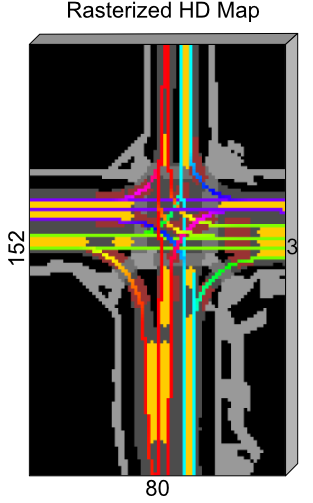
\includegraphics[width=\textwidth]{figures/caspnet-bev-repr.png}
    \caption{Rasterized BEV encoding}
    \label{fig:rasterized}
\end{subfigure}
\hfill
\begin{subfigure}[t]{0.37\textwidth}
    \centering
    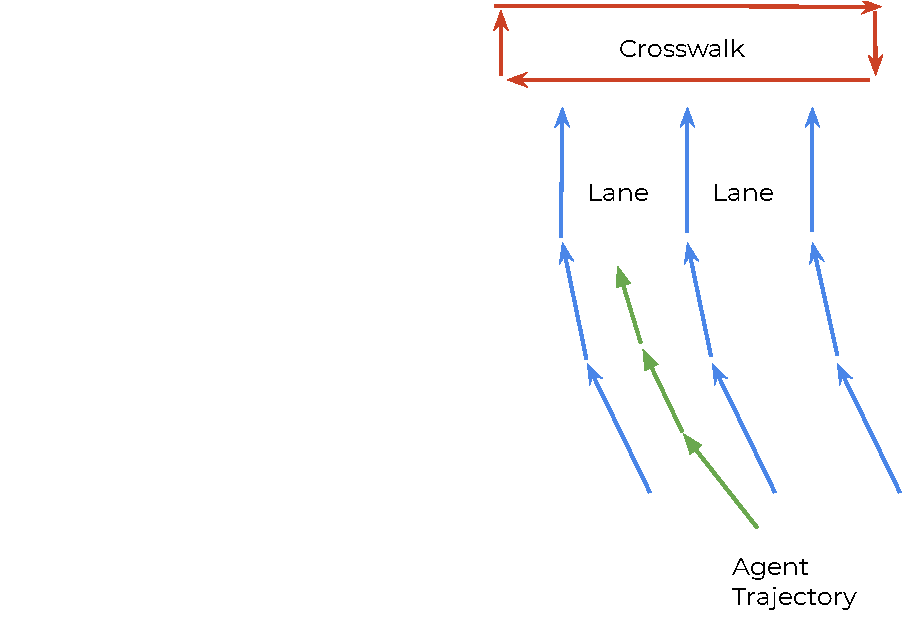
\includegraphics[width=\textwidth]{figures/vectornet-2020-vector-repr.pdf}
    \caption{Vectorized polyline preservation}
    \label{fig:vectorized}
\end{subfigure}
\caption{Scene representation paradigms in trajectory prediction: (a) rasterized approaches stack agent trajectories and HD maps into BEV images~\cite{caspnetSchäfer2022}, (b) vectorized methods preserve geometric polylines~\cite{gao2020vectornet}.}
\label{fig:scene_representations}
\end{figure}

% TODO: use \begin{description}
%   \item[]
% \end{description} instead of textbf{} to introduce the two paradigms

\begin{description}
\item[Raster grids.] Early systems stack past agent masks and HD-map layers into \( F \)-dimensional BEV (Bird's Eye View) images, leveraging convolutional backbones to capture spatial relationships while keeping runtime independent of the number of agents~\cite{cui2019multimodal,chai2019multipath}. Specifically, these approaches construct: (i) a BEV stack of past agent trajectories \( \mathbf{I}_d\in\R^{T_p\times H\times W\times F_d} \) and (ii) a static HD-map raster \( \mathbf{I}_s\in\R^{H\times W\times F_s} \).\\
The CASPNet family of motion forecasting models, consisting of the original CASPNet~\cite{caspnetSchäfer2022}, which utilizes a fully convolutional architecture, CASPNet++~\cite{caspnetppSchäfer2023}, and the CASPFormer~\cite{caspformerYadav2024}, exemplifies interesting architectural choices within this paradigm and will be discussed in greater detail in~\autoref{ssec:caspnet}.\\
However, rasterized approaches suffer from limited geometric fidelity and redundant pixel information due to grid-based discretization of scene elements' geometric and kinematic properties~\cite{lmformerYadav2025}. Additionally, respecting agent identities is infeasible as it would require separate channels per agent, introducing further redundancy; CASPNet++~\cite{caspnetppSchäfer2023} addressed this using single BEV per agent. Furthermore, rasterized approaches allow only shared coordinate systems, which is suboptimal for leveraging geometric isomorphisms~\cite{qcnetZhou2023}. % TODO: it is infeasible to respect the identities of agents as this would require a separate channel or set of channels for each agent throughout the entire architecture, which would introduce even more redundancy in terms of pixel information. However, respecting identities is crucial for true multi-agent motion forecasting, the aforementioned approach of using a single BEV per agent was used in \cite{caspnetppSchäfer2023}. Additionally, rasterized approaches allow only a shared coordinate system, which is suboptimal in terms of leverageable geometric isomorphisms.

\item[Vector representations.] Later work encodes agents and lanes as vectorized geometric primitives such as polylines, enabling graph (LaneGCN~\cite{liang2020learning}, VectorNet~\cite{VectorNet2020}) or transformer based (QCNet~\cite{qcnetZhou2023}, QCNeXt~\cite{qcnextZhou2023}, LMFormer~\cite{lmformerYadav2025}) approaches with higher geometric fidelity but runtime that grows with scene complexity. These representations are more compact, preserve higher geometric fidelity, and enable explicit modeling of complex spatio-temporal and social relationships between scene elements. Lane information uses two main representations:
\begin{itemize}
  \item \textbf{Point-based}: Each polyline \(L_p^i = [P_1^i, P_2^i, \ldots, P_K^i]\) with \(K\) control points \(P_k^i\)~\cite{VectorNet2020, zhou2022hivt}.
  \item \textbf{Segment-based}: Converts to \(L_v^i = [V_1^i, V_2^i, \ldots, V_{K-1}^i]\) where \(V_{k}^i = [P_k^i, P_{k+1}^i]\) stores lane segment vectors. This explicitly encodes road curvature~\cite{liang2020learning,zhou2022hivt,qcnetZhou2023}.
\end{itemize}
Agent trajectories use analogous representations:
\begin{itemize}
  \item \textbf{Trajectory points}: \(\mathcal{T}_{in}^a = [P_1^a, P_2^a, \ldots, P_T^a]\) with global positions \(P_t^a\).
  \item \textbf{Motion vectors}: \(M_t^a = [P_{2}^a - P_{1}^a, \ldots, P_{T}^a - P_{T-1}^a]\) derived from trajectories, representing the displacement between timesteps~\cite{lmformerYadav2025}.
\end{itemize}
Vectorized approaches employ either \emph{agent-centric} coordinate systems (all scene elements normalized to a single ego-centric frame) or \emph{query-centric}~\cite{qcnetZhou2023} paradigms. The choice fundamentally affects computational efficiency, invariance properties, and multi-agent reasoning capabilities, with query-centric approaches offering significant advantages for streaming applications and parallel multi-agent prediction. % TODO: introduce the Vector Based Representation by saying that they are more compact and preserve more geometric fidelity, they are more appropriate for the use in transformer or graph based approaches and allow to model complex spatio-temporal and social relationships between scene elements more explicitly. % TODO: elaborate more closely what agent-centric means: i.e. a single ego-centric coordinate system for all agents.
\end{description}

% This so-called \emph{query-centric} approach will be discussed in greater detail in~\autoref{ssec:qc_paradigm}. CASPNet embodies the \emph{raster} philosophy; CASPFormer adopts a hybrid strategy—retaining a CNN backbone for perception compatibility, but switching to a vectorized transformer decoder for output precision.

\subsubsection{The Query-Centric Paradigm}
\label{ssec:qc_paradigm}

QCNet generalizes vector-based encoders by abandoning a single ego-centric grid in favor of local `fibers' for every map polygon or agent-state, yielding strict roto-translation and temporal invariance while enabling streaming-time reuse~\cite{qcnetZhou2023}. Each map polygon and each agent \emph{state} owns a local spacetime frame \((p,\theta,t)\) (Fig.~\ref{fig:polar-frames-three}). All geometry is expressed in these frames; relative descriptors \([\lvert\lvert p_j-p_i\rvert\rvert_2,\;\Delta\theta_{\text{dir}},\;\Delta\theta_{\text{ori}},\;\Delta t]\) are Fourier-MLP embedded and concatenated to keys/values in factorised attention. Consequently the scene tensor is \textbf{roto-translation \& time invariant}, can be \textbf{cached across sliding windows}, and is \textbf{shared by every target agent}, lowering online complexity from \(O(AT^2)\) to \(O(AT)\)~\cite{qcnetZhou2023}.
\begin{figure}[ht]
\centering
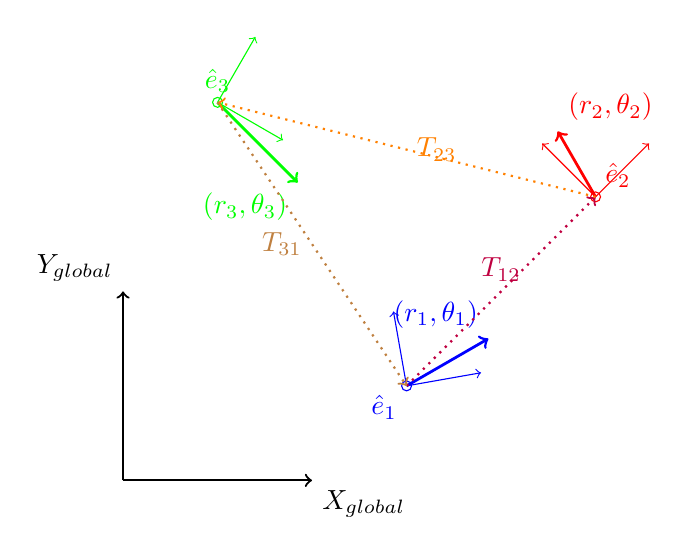
\begin{tikzpicture}[scale=1.2]
  % Global Cartesian axes
  \draw[thick,->] (0,0) -- (2,0) node[anchor=north west]{$X_{global}$};
  \draw[thick,->] (0,0) -- (0,2) node[anchor=south east]{$Y_{global}$};

  % Global positions of elements
  \coordinate (e1) at (3,1);
  \coordinate (e2) at (5,3);
  \coordinate (e3) at (1,4);

  % Local origins (fibers) marked as filled dots
  \draw[blue,fill=white]  (e1) circle(1.5pt) node[below left] {$\hat e_1$};
  \draw[red,fill=white]   (e2) circle(1.5pt) node[above right] {$\hat e_2$};
  \draw[green,fill=white] (e3) circle(1.5pt) node[above] {$\hat e_3$};

  % Local reference frames (Cartesian axes) at each origin
  \draw[blue,thin,->]  (e1) -- ++(10:0.8)  node[anchor=south] {};
  \draw[blue,thin,->]  (e1) -- ++(100:0.8) node[anchor=west] {};

  \draw[red,thin,->]   (e2) -- ++(45:0.8)  node[anchor=south west] {};
  \draw[red,thin,->]   (e2) -- ++(135:0.8) node[anchor=north] {};

  \draw[green,thin,->] (e3) -- ++(-30:0.8) node[anchor=east] {};
  \draw[green,thin,->] (e3) -- ++(60:0.8)  node[anchor=west] {};


  % Local motion vectors in polar form with varying length and rotation
  \draw[blue,->,line width=1pt]  (e1) -- ++( 30:1.0) node[anchor=south east] {$(r_1,\theta_1)$};
  \draw[red,->,line width=1pt]   (e2) -- ++(120:0.8) node[anchor=south west] {$(r_2,\theta_2)$};
  \draw[green,->,line width=1pt] (e3) -- ++(-45:1.2) node[anchor=north east] {$(r_3,\theta_3)$};

  % Relative transforms between elements
  \draw[purple,dotted,->,thick] (e1) -- (e2) node[midway,above] {$T_{12}$};
  \draw[orange,dotted,->,thick] (e2) -- (e3) node[midway,right] {$T_{23}$};
  \draw[brown,dotted,->,thick]  (e3) -- (e1) node[midway,left] {$T_{31}$};
\end{tikzpicture}
\caption{Query-centric layout with global Cartesian axes, annotated motion vectors \((r_i,\theta_i)\) for each element \(\hat e_1,\hat e_2,\hat e_3\), and relative transforms \(T_{12}\), \(T_{23}\), \(T_{31}\). Each local origin (fiber) is shown as a filled dot.}
\label{fig:polar-frames-three}
\end{figure}

\begin{figure}[ht]
\centering
\begin{tikzpicture}[scale=1.2]
  % Origins
  \coordinate (e1) at (0,0);
  \coordinate (e2) at (3,1.5);

  % 1) Euclidean distance between origins
  \draw[black,->,thick] (e1) -- node[above] {\(d=\lvert\lvert p_j-p_i\rvert\rvert\)} (e2);

  % Frame at e_i
  \draw[blue,->,>=Stealth,line width=1pt]    (e1) -- ++(0:1)    node[below right] (e1x) {$x_i$};
  \draw[blue,->,>=Stealth,line width=1pt]    (e1) -- ++(90:1)   node[above left]  (e1y) {$y_i$};
  \draw[blue,fill=white,draw,inner sep=1pt,circle] (e1) node[below left] {$\hat e_i$};
  % Motion vector in frame i
  \draw[blue,->,>=Stealth,line width=1pt] (e1) -- ++(30:1.2) node[midway,above right] {$(r_i,\theta_i)$};

  % Frame at e_j
  \draw[red,->,>=Stealth,line width=1pt]     (e2) -- ++(40:1)   node[above right] (e2x) {$x_j$};
  \draw[red,->,>=Stealth,line width=1pt]     (e2) -- ++(130:1)  node[above left]  (e2y) {$y_j$};
  \draw[red,fill=white,draw,inner sep=1pt,circle]    (e2) node[below right] {$\hat e_j$};
  % Motion vector in frame j
  \draw[red,->,>=Stealth,line width=1pt] (e2) -- ++(100:1) node[midway,above left] {$(r_j,\theta_j)$};

  % 2) Angle between the two x-axes: Δθ_axes at e1
  \pic [draw=black,densely dashed,->,>=Stealth,angle radius=8mm,"$\Delta\theta_{\mathrm{axes}}$"{font=\footnotesize,fill=white,inner sep=1pt}]
       {angle = e1x--e1--e2x};

  % 3) Relative angle between motion vectors: Δθ_motion at e2
  % First define the copy of e1's motion direction at e2
  \coordinate (u2) at ($(e2)+(30:1.2)$);
  % Now angle pic between that and e2's motion vector
  \pic [draw=black,densely dashed,->,>=Stealth,angle radius=8mm,"$\Delta\theta_{\mathrm{motion}}$"{font=\footnotesize,fill=white,inner sep=1pt}]
       {angle = u2--e2--e2y}; % note: use e2y if v2 wasn't named

\end{tikzpicture}
\caption{Query-centric spatial descriptors between elements \(i\) and \(j\):
(1) Euclidean distance \(d=\lvert\lvert p_j-p_i\rvert\rvert\);
(2) orientation difference of local \(x\)-axes \(\Delta\theta_{\mathrm{axes}}=\theta_j-\theta_i\);
(3) relative angle between their motion vectors \(\Delta\theta_{\mathrm{motion}}=\theta_j^{\mathrm{motion}}-\theta_i^{\mathrm{motion}}\).}
\label{fig:qc_spatial_descriptors}
\end{figure}

\subsubsection*{Integration with Modern Architectures}
The query-centric paradigm has been successfully integrated with various modern deep learning architectures:

\begin{itemize}
    \item \textbf{Transformer-based models:} QCNet and QCNeXt demonstrate the natural synergy between query-centric encoding and attention mechanisms.
    \item \textbf{Graph neural networks:} The paradigm can be adapted for GNN-based trajectory prediction by treating each element's local frame as a node feature.
\end{itemize}

In summary, the query-centric paradigm provides a principled, symmetry-respecting, and efficient foundation for trajectory forecasting. The combination of local polar encodings and relative descriptors yields a flexible and lossless representation, underpinning the success of recent state-of-the-art models. This approach has fundamentally changed how the community thinks about scene representation for autonomous driving, moving from agent-centric to truly democratic, multi-agent reasoning systems.



\newpage